% This file is part of the package
%
% "Teaching material for the subject 'Fachinformatik' at German vocational schools"
%
% (c) 2024 Hohenahr/Germany: Karsten Reincke
%
% All files of the uninstantiated package are distributed under the terms of the 
% creative commons license CC-BY-4.0 (= https://creativecommons.org/licenses/by/4.0/)
%
% Instantiated files referring to specific classes / persons / pupils may only be
% distributed within the teaching staff of the 'Gewerbliche Schule Lahn-Dill-Kreis'
%

\selectlanguage{ngerman}

\begin{frame}
  \frametitle{LF09:04:Repeater und Hub}
  \begin{center}
  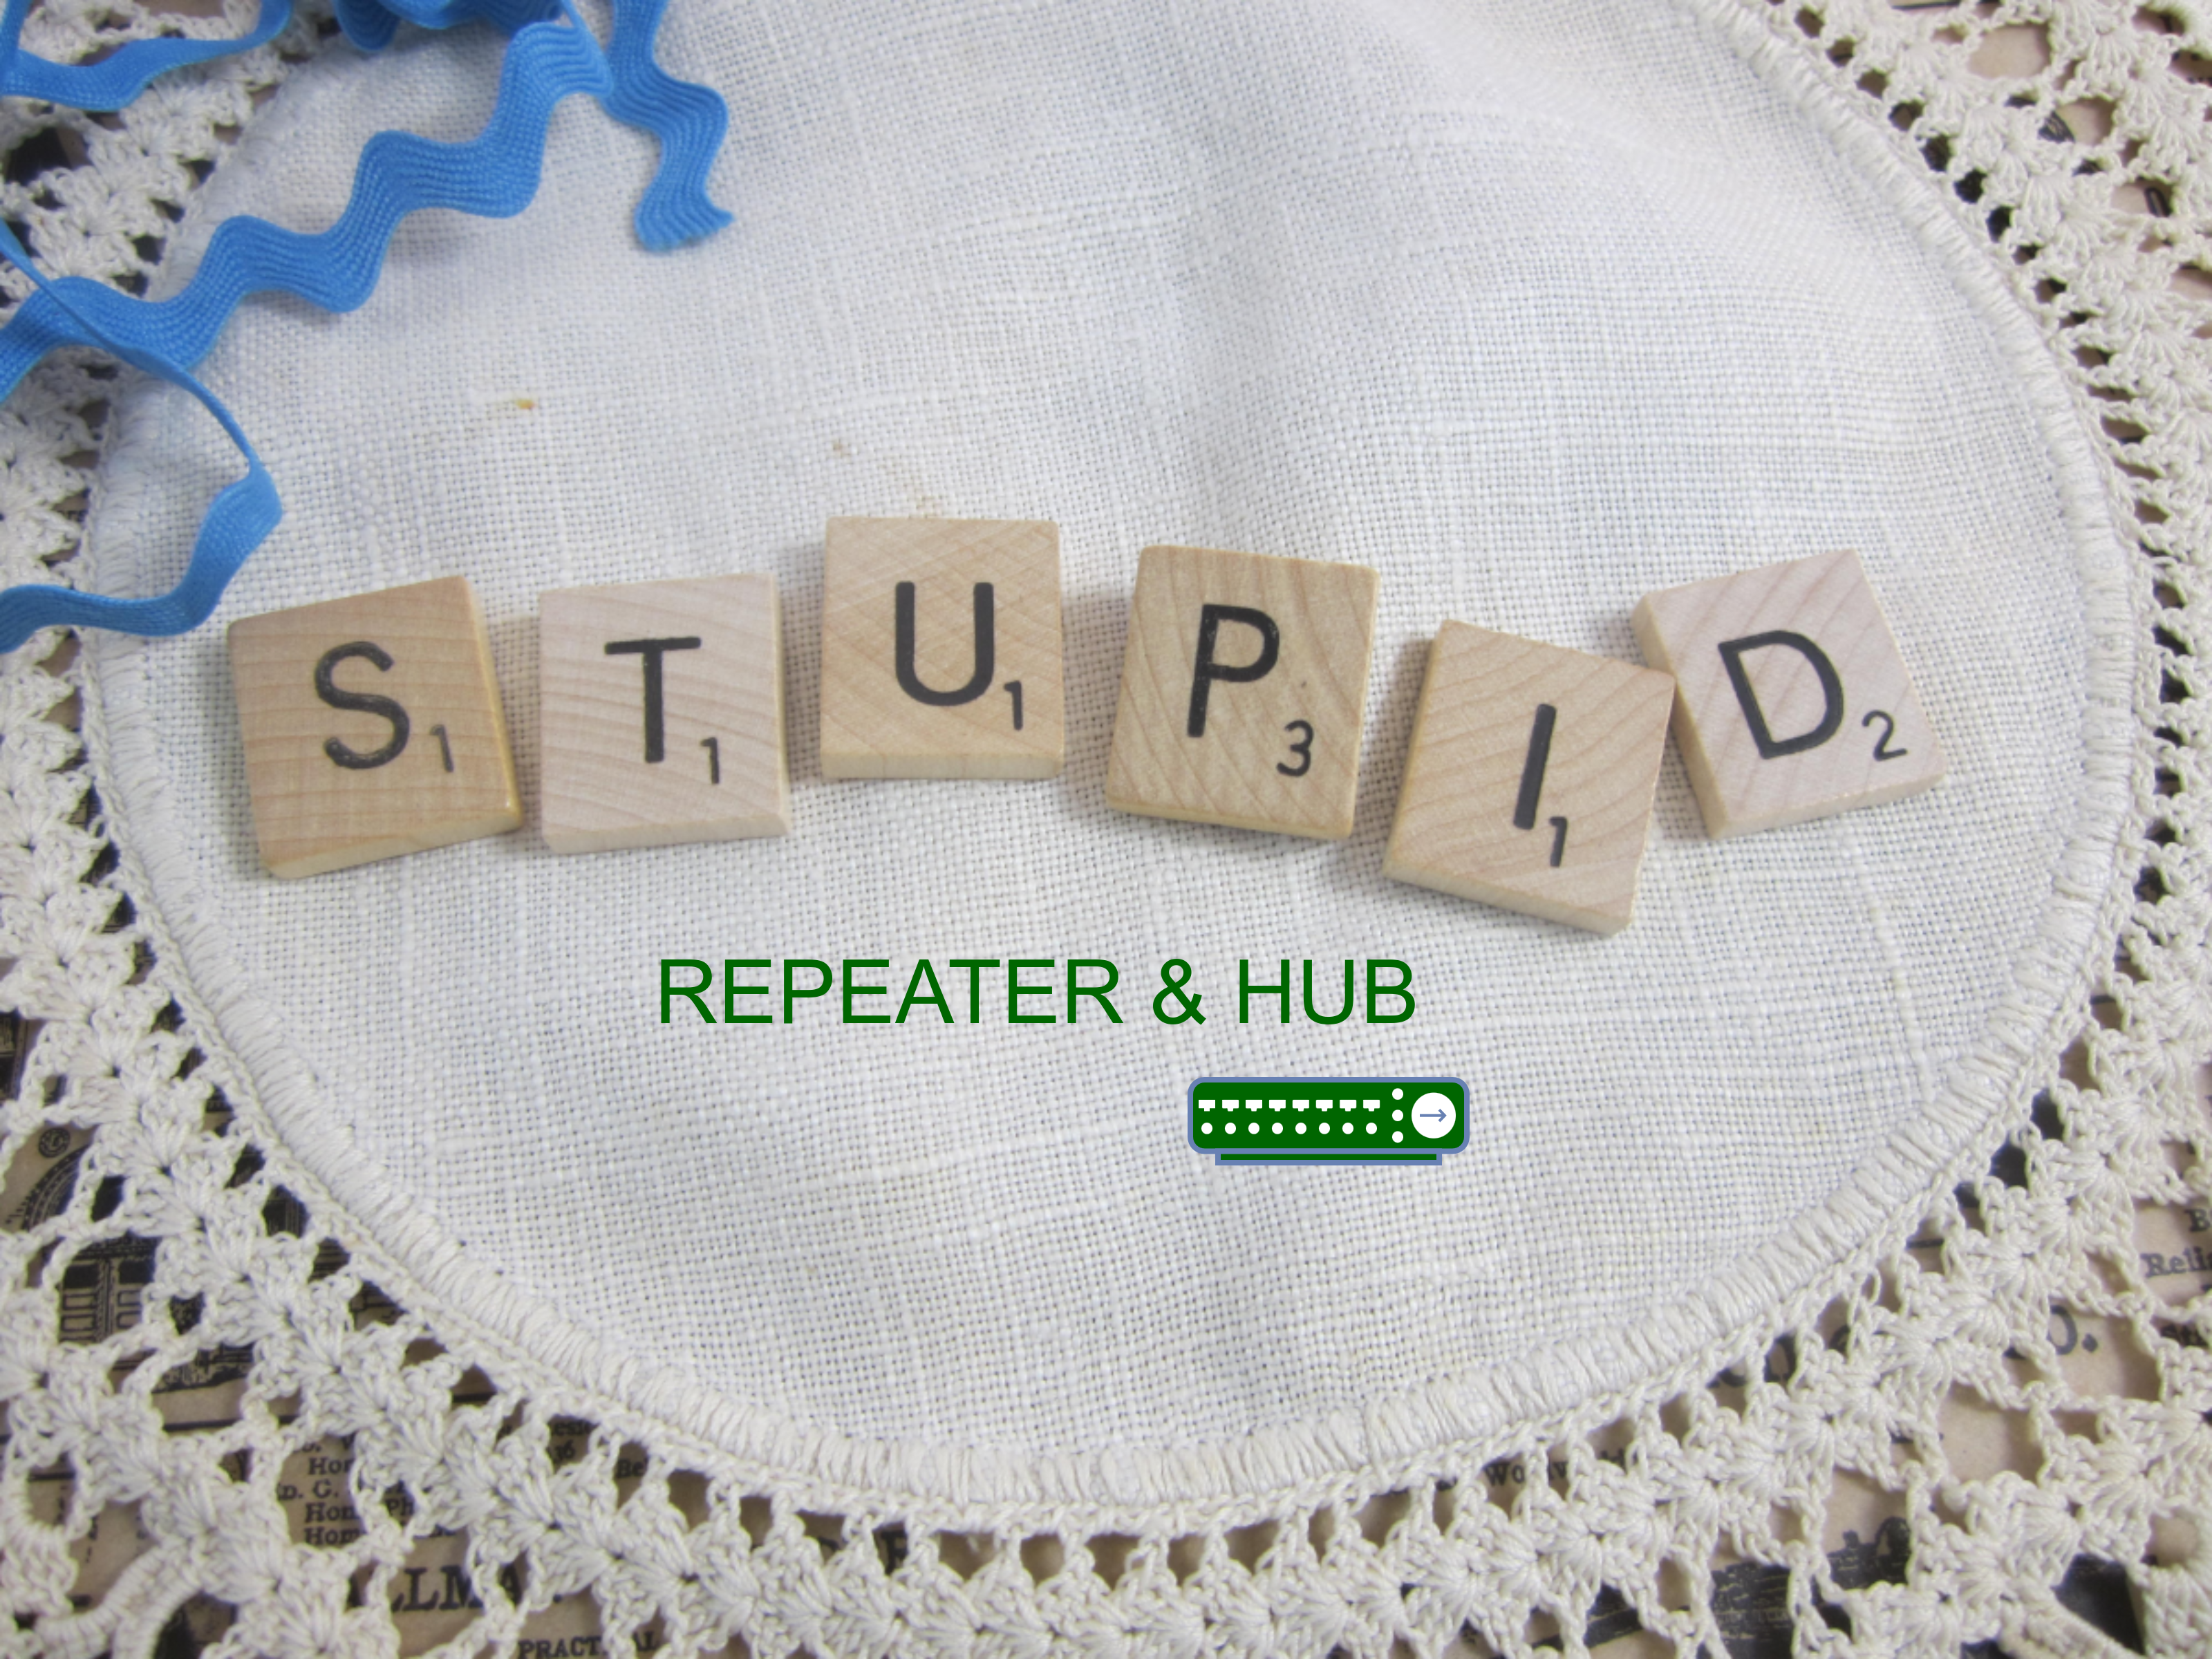
\includegraphics[height=7cm]{\imgLf/arp-stupid-repeater-hub.png}
  \end{center}
\end{frame}

\begin{frame}
  \frametitle{LF09:04:Hub-Netz}
  \begin{center}
  \includegraphics[height=7cm]{\imgLf/arp-hub-network.png}
  \end{center}
\end{frame}

\begin{frame}
  \frametitle{LF09:04:ARP-Paketstruktur}
  \begin{center}
  \includegraphics[height=7cm]{\imgLf/arp-package-structure.png}
  \end{center}
\end{frame}

\begin{frame}
  \frametitle{LF09:04:Hub-Netz:ARP-Aktivitätsdiagramm}
  \begin{center}
  \includegraphics[height=7.5cm]{\imgLf/arp-hub-activity.png}
  \end{center}
\end{frame}

\begin{frame}
\frametitle{LF09:04:Hub-Netz:ARP-Sequenzdiagramm}
\begin{center}
\includegraphics[height=7.5cm]{\imgLf/arp-hub-sequence.png}
\end{center}
\end{frame}

\begin{frame}
\frametitle{LF09:04:Hub-Netz:ARP-Schreibtischtest}
\begin{center}
\includegraphics[height=6cm]{\imgLf/arp-desk-test.png}
\end{center}
\end{frame}

\begin{frame}
\frametitle{LF09:04:Hub-Netz:ARP-Probleme}
\begin{center}
\includegraphics[height=6cm]{\imgLf/collision-1019693-pxh.png}
\end{center}
\end{frame}

\begin{frame}
  \frametitle{LF09:04:Hub-Netz:ARP-Revision}
  \begin{columns}[t]
    \column{0.3\textwidth}
    \textbf{beibehalten:}
    \begin{itemize}
      \item Austauschbarkeit
      \item Erweiterbarkeit
      \item (Re)Startbarkeit
      \item günstige Lösung
    \end{itemize}
    \column{0.4\textwidth}
    \textbf{verbessern:}
    \begin{itemize}
      \item weniger Kollisionen 
      \item weniger Nachrichten
      \item weniger Relevanzanalysen
      \item größere Netze    
    \end{itemize}
    \column{0.2\textwidth}
      \begin{center}
        \includegraphics[height=1cm]{\imgLf/collision-1019693-pxh.png}
      \end{center}
  \end{columns}
\end{frame}



